\documentclass[11pt,a4paper]{article}
\usepackage[margin=1.1in]{geometry}
\usepackage{amsmath,amssymb,amsthm}
\usepackage{booktabs}
\usepackage{graphicx}
\usepackage[round]{natbib}
\usepackage[hidelinks]{hyperref}
\hypersetup{
  pdftitle={How Much Data Does an Information Coefficient Need? The Sampling Distribution of a Cross-Sectional IC, and Why Breadth Does Not Buy Precision},
  pdfauthor={Himal Naidu},
  pdfsubject={Statistical power and effective sample size of the cross-sectional information coefficient},
  pdfkeywords={information coefficient, statistical power, effective sample size, fundamental law of active management, factor models, replication}
}
\usepackage{microtype}
\setlength{\emergencystretch}{1.5em}  % lets the long repo URL wrap instead of overflowing

% Generated by tools/make_numbers.py -- do not edit.
% Every estimate in paper.tex comes from data/results.json via these macros.
\newcommand{\panelStart}{2000-02}
\newcommand{\panelEnd}{2026-02}
\newcommand{\nTickers}{2{,}559}
\newcommand{\panelObs}{465{,}750}
\newcommand{\momT}{300}
\newcommand{\momMean}{0.0123}
\newcommand{\momSd}{0.1411}
\newcommand{\momTstat}{1.51}
\newcommand{\momTnw}{1.60}
\newcommand{\momAR}{-0.02}
\newcommand{\momKurt}{3.82}
\newcommand{\momN}{1{,}552}
\newcommand{\momNeff}{50}
\newcommand{\momPlacebo}{0.0766}
\newcommand{\momPlaceboRatio}{3.0}
\newcommand{\revT}{312}
\newcommand{\revMean}{0.0221}
\newcommand{\revSd}{0.1164}
\newcommand{\revTstat}{3.36}
\newcommand{\revTnw}{3.56}
\newcommand{\revAR}{-0.06}
\newcommand{\revNeff}{74}
\newcommand{\revN}{1{,}570}
\newcommand{\revPlacebo}{0.0689}
\newcommand{\momFloor}{0.1397}
\newcommand{\momC}{1.090}
\newcommand{\momCeil}{51}
\newcommand{\revFloor}{0.1136}
\newcommand{\revC}{1.097}
\newcommand{\revCeil}{77}
\newcommand{\randFloorVar}{0.000042}
\newcommand{\randC}{1.023}
\newcommand{\momFloorVar}{0.019514}
\newcommand{\momOvershoot}{9}
\newcommand{\neffOneK}{48.7}
\newcommand{\neffTwoK}{50.0}
\newcommand{\randMaxDev}{3}
\newcommand{\iidNull}{0.0254}
\newcommand{\cohortN}{1{,}083}
\newcommand{\cohortMean}{0.0040}
\newcommand{\cohortSd}{0.1539}
\newcommand{\cohortSdChange}{9}
\newcommand{\pearsonMean}{-0.0080}
\newcommand{\pearsonSd}{0.1410}
\newcommand{\simTrueIC}{0.0296}
\newcommand{\simFloor}{0.008884}
\newcommand{\simFloorSd}{0.0943}
\newcommand{\simClosed}{0.010115}
\newcommand{\simNaive}{0.011025}
\newcommand{\simFit}{0.008807}
\newcommand{\simFitSe}{0.000063}
\newcommand{\simFitC}{0.997}
\newcommand{\simKappa}{0.972}
\newcommand{\simFitCSe}{0.014}
\newcommand{\simKappaUErr}{5}
\newcommand{\simClosedErr}{14.9}
\newcommand{\simNaiveErr}{25.2}
\newcommand{\simExactErr}{0.9}
\newcommand{\simExactSig}{1.2}
\newcommand{\simClosedSig}{20.7}
\newcommand{\simNaiveSig}{35.1}
\newcommand{\sigmaIC}{0.141}
\newcommand{\effObs}{15{,}078}
\newcommand{\neededObs}{8{,}721}
\newcommand{\overstate}{31}
\newcommand{\reqTbonferronithreezerozero}{468}
\newcommand{\reqYbonferronithreezerozero}{39.0}
\newcommand{\reqThlz}{326}
\newcommand{\reqYhlz}{27.2}
\newcommand{\reqTsingle}{174}
\newcommand{\reqYsingle}{14.5}
\newcommand{\mdefive}{0.0510}
\newcommand{\mdeonezero}{0.0361}
\newcommand{\mdetwozero}{0.0255}
\newcommand{\mdetwofive}{0.0228}
\newcommand{\mdefiveseven}{0.0151}
\newcommand{\typemfive}{1.61}
\newcommand{\typemonezero}{1.25}
\newcommand{\typemtwozero}{1.05}
\newcommand{\typemtwofive}{1.03}
\newcommand{\typemfiveseven}{1.00}
\newcommand{\covonetwozero}{0.951}
\newcommand{\covtwofour}{0.936}
\newcommand{\covthreezerozero}{0.952}
\newcommand{\covsixzero}{0.946}
\newcommand{\pwsimonetwozero}{0.876}
\newcommand{\pwanaonetwozero}{0.861}
\newcommand{\pwsimtwofour}{0.308}
\newcommand{\pwanatwofour}{0.275}
\newcommand{\pwsimthreezerozero}{0.999}
\newcommand{\pwanathreezerozero}{0.998}
\newcommand{\pwsimsixzero}{0.585}
\newcommand{\pwanasixzero}{0.576}
\newcommand{\simrows}{%
50 & 0.029022 & 0.028325 & $-2.4\%$ \\
100 & 0.018320 & 0.018605 & $+1.6\%$ \\
200 & 0.013642 & 0.013745 & $+0.8\%$ \\
400 & 0.011296 & 0.011314 & $+0.2\%$ \\
800 & 0.010010 & 0.010099 & $+0.9\%$ \\
1600 & 0.009510 & 0.009492 & $-0.2\%$ \\
3200 & 0.009208 & 0.009188 & $-0.2\%$ \\
12800 & 0.009107 & 0.008960 & $-1.6\%$ \\}
\newcommand{\breadthrows}{%
50 & 0.2021 & 0.1866 & 0.1428 & 0.1429 \\
100 & 0.1778 & 0.1548 & 0.1025 & 0.1005 \\
200 & 0.1565 & 0.1354 & 0.0715 & 0.0709 \\
400 & 0.1485 & 0.1255 & 0.0514 & 0.0501 \\
800 & 0.1441 & 0.1191 & 0.0358 & 0.0354 \\
1000 & 0.1436 & 0.1185 & 0.0311 & 0.0316 \\
\midrule
fitted $\sF$ & 0.1397 & 0.1136 & $\approx 0$ & --- \\
fitted $c$ & 1.090 & 1.097 & 1.023 & --- \\}
                    % generated from data/results.json; never edited

\newtheorem{proposition}{Proposition}
\newcommand{\ICh}{\widehat{IC}}
\newcommand{\Neff}{N_{\mathrm{eff}}}
\newcommand{\sF}{\sigma_F}

\title{\bfseries How Much Data Does an Information Coefficient Need?\\[0.35em]
\large The Sampling Distribution of a Cross-Sectional IC,\\ and Why Breadth Does Not Buy Precision}
\author{Himal Naidu\\[0.2em]
\normalsize Independent Researcher\\
\normalsize \href{mailto:thotahimalnaidu@gmail.com}{\texttt{thotahimalnaidu@gmail.com}}}
\date{October 2026}

\begin{document}
\maketitle

\begin{abstract}
\noindent
A cross-sectional information coefficient (IC) is usually treated as if the stocks in
each period were an independent sample, so that $N$ stocks give a standard error of
order $1/\sqrt{N}$. Any real signal is correlated with factor loadings, though, so each
period's IC also picks up that period's factor return, a single draw shared by every
stock. I show that $\mathrm{Var}(\ICh_t) = \sF^2 + \kappa/N$ with $\kappa \approx 1$,
where the floor $\sF^2$ does not shrink as stocks are added, so effective sample size is
capped at $1/\sF^2$. Simulation confirms the formula. On \nTickers{} US stocks over
\panelStart{}--\panelEnd{}, the IC volatility of $12-1$ momentum levels off at
$\sF = \momFloor$: a cross-section of $\momN$ names is worth about $\momNeff$ independent
observations, while a randomly permuted signal follows the classical formula. Detecting
a true IC of $0.03$ at $80\%$ power takes \reqYsingle{} years of monthly data, or
\reqYhlz{} years at the $t>3$ hurdle, and no ten-year window is long enough. The floor
itself is the strategy risk of \citet{qian2004active}; what this paper adds is what it
means for inference.

\medskip
\noindent\textbf{Keywords:} information coefficient, statistical power, effective sample
size, fundamental law of active management, factor models, replication

\noindent\textbf{JEL classification:} C12, C15, G11, G12
\end{abstract}

\section{Summary in plain language}

An investor who thinks they can predict which stocks will do well might test it like
this. Each month, score every stock, wait a month, and check whether the high-scoring
stocks actually did better. The correlation between the scores and what happened is
called the information coefficient. Averaged over years of
monthly data, published figures are often around $0.03$. That is a weak relationship (a perfect forecast would score $1$), but
applied to thousands of stocks every month it is enough to run a business on.

How sure can anyone be that a measured $0.03$ is real and not luck? The obvious answer
is: very sure. Two thousand stocks a month for twenty-five years is about half a
million observations. This paper shows why that answer is wrong and works out by how
much.

Stocks do not move independently. In any month a few big shared movements push every
stock at once: the whole market rises, say, or cheap stocks beat expensive ones. And
any signal a person would actually use is related to which stocks are exposed to those
movements. Recent winners tend to be the jumpier stocks; cheap stocks tend to be the
riskier ones. So part of each month's measured correlation just reflects which way
the market happened to lean that month.

Adding more stocks does not fix this, because there is only one market movement per
month and it touches everything. Noise that is specific to individual companies washes out as names are added; the shared part does not.

I work out how large the shared part is, check the formula on simulated data where the
right answer is known, and then measure it on twenty-five years of US stock prices. A
cross-section of about $\momN$ stocks turns out to carry as much information as roughly
$\momNeff$ independent observations.

Showing that a true information coefficient of $0.03$ is different from zero takes about \reqYsingle{} years of monthly data, or about \reqYhlz{} years under the stricter
standard the field now uses because so many strategies have been tried. Over any
ten-year stretch the smallest effect that can be reliably detected is $\mdeonezero$, which is
larger than $0.03$. A study that reports such an effect ``holds in every decade'' is
claiming more than its data can show.

Momentum (buying stocks that have risen over the past year) gives an average IC of
$\momMean$ over \momT{} months in my data, with a $t$-statistic of $\momTstat$, which
is not distinguishable from zero.

\section{Motivation}

The information coefficient is the standard summary statistic for a return-predicting
signal, in academic work and in industry. It is reported constantly and its precision is
reported rarely. When a standard error does accompany it, the usual construction is
Fama--MacBeth: treat the $T$ per-period ICs as a sample and use
$t = \sqrt{T}\,\overline{IC}/\hat\sigma_{IC}$ \citep{fama1973risk}. The procedure is sound;
the problem is the intuition about how much precision the cross-section supplies.

For $N$ independent pairs, the sample correlation has a standard error of about
$1/\sqrt{N-1}$. With $N = 2000$ that
is $0.022$; averaged over $T = 300$ months it becomes $0.0013$, which puts an IC of
$0.03$ about $23$ standard errors from zero. Under this arithmetic no cross-sectional IC of
plausible magnitude could ever fail to be significant, and questions of statistical power
never arise.

Several facts do not fit this picture. Realised IC series have standard deviations
around $0.10$--$0.15$, five or six times the classical figure. Practitioners have long
treated the volatility of the IC as a risk in its own right \citep{qian2004active}. And
the empirical anomaly literature has the kind of replication problem that low power
produces: \citet{hou2020replicating} find
that $65\%$ of $452$ anomalies fail to clear $|t| > 1.96$ once microcaps are handled,
rising to $82\%$ at a multiple-testing hurdle, and that surviving effects are typically
much smaller than first reported. \citet{mclean2016academic} document returns $26\%$
lower out of sample and $58\%$ lower after publication.

I derive the sampling distribution of the
cross-sectional IC under a factor model, check it by simulation, and measure its
parameters on real data. The result turns the vague sense that ICs are noisy into a
sample-size requirement that any particular study can be checked against.
Section~\ref{sec:related} sets out which parts of this are already known.

\section{Related work}\label{sec:related}

\paragraph{The fundamental law, and what it already contains.}
\citet{grinold1989law} gave the fundamental law of active management,
$IR \approx IC \cdot \sqrt{BR}$, with $BR$ the number of independent bets. The law is
about attainable performance, not about estimation, but its breadth term is the source
of the intuition this paper contradicts. \citet{clarke2002constraints} added the transfer
coefficient to account for the information lost to portfolio constraints.

Two papers come closest. \citet{qian2004active} showed that the volatility of the IC
through time is a separate, non-diversifiable component of active risk, which they
named \emph{strategy risk}, and proposed the ratio of mean IC to IC standard deviation
as the right performance statistic. Those are the same two moments whose sampling
behaviour I study. \citet{ding2017redux} then derived a fundamental law in which the information
ratio is increasing in the mean of $IC_t$, decreasing in its volatility, and subject to
an absolute upper bound as $N \to \infty$.

The existence of a non-diversifiable component of IC variance is therefore not my
finding; it
is in both papers. What they do not cover is the inference side: the sampling
distribution of $\overline{IC}$, an effective sample size for a cross-section, and the
number of periods needed before a claimed IC can be distinguished from zero. Ding and
Martin answer a portfolio-construction question (how good can a manager get?), and I
answer an inference question (how much data does a claim need?), using the same
variance term.

\paragraph{What sets precision in cross-sectional tests.}
\citet{ang2020stocks} show that the precision of cross-sectional risk-premium estimates
depends on the cross-sectional dispersion of factor loadings: grouping stocks into
portfolios estimates each beta more precisely but shrinks that dispersion, and the
standard errors of the risk premia get larger. \citet{lewellen2010skeptical} make a
related point about the apparent success of asset pricing models on portfolios with
strong factor structure. My setting is related. Here too the precision of a
cross-sectional estimate depends on the structure of the cross-section, and counting
assets overstates it once a common component is present.

\paragraph{Multiple testing and replication.}
\citet{harvey2016cross} argue that the sheer number of factors tested requires a hurdle
of about $t > 3.0$ rather than $1.96$. \citet{hou2020replicating} document the resulting
replication failures, and \citet{chen2022opensource} provide an open catalogue of $319$
published predictors, which fixes the order of magnitude of the multiple-testing problem.
\citet{chen2021phacking} argues that $p$-hacking alone cannot account for the largest
published $t$-statistics. This literature asks whether a given significance threshold is
strict enough. I ask an earlier question, whether a study has the power to reach any
threshold at all. The two interact: a stricter hurdle raises the required sample.

\paragraph{Power and magnitude errors.}
Outside finance, \citet{ioannidis2005why} argued that low power makes a large share of
published positive findings false, and \citet{gelman2014beyond} showed that it also
inflates the published magnitudes of effects that are real. I use Gelman and Carlin's
exaggeration ratio in \S\ref{sec:typem}.

\section{Setup}\label{sec:setup}

Fix a rebalancing date $t$ with $N$ assets. Let $s_{i,t}$ be the signal, standardised
cross-sectionally so that $\mathrm{mean}_i(s) = 0$ and $\mathrm{var}_i(s) = 1$, and let
$r_{i,t+1}$ be the return earned over the following period. The realised IC is the
cross-sectional correlation
\begin{equation}
\ICh_t \;=\; \frac{\mathrm{cov}_i(s_{\cdot,t},\, r_{\cdot,t+1})}{\mathrm{sd}_i(r_{\cdot,t+1})},
\label{eq:icdef}
\end{equation}
and the reported statistic is $\overline{IC} = T^{-1}\sum_{t=1}^{T}\ICh_t$. Throughout,
$\mathrm{mean}_i$, $\mathrm{cov}_i$ and $\mathrm{sd}_i$ denote moments taken across
assets at a fixed date; expectations and variances without a subscript are over repeated
draws of the return process.

Returns follow a one-factor model,
\begin{equation}
r_{i,t+1} \;=\; \lambda s_{i,t} \;+\; \beta_i f_{t+1} \;+\; \varepsilon_{i,t+1},
\label{eq:model}
\end{equation}
with $f_{t+1}$ the factor return, $\mathrm{var}(f) = \sigma_f^2$; $\varepsilon$
cross-sectionally uncorrelated with variance $\sigma_\varepsilon^2$ and independent of
$f$; and $\lambda \geq 0$ the strength of genuine predictability. Write
$v_\beta = \mathrm{var}_i(\beta)$ and
\begin{equation}
q \;\equiv\; \mathrm{cov}_i(s_{\cdot,t},\, \beta_\cdot),
\label{eq:q}
\end{equation}
the cross-sectional covariance between the signal and the factor loadings. Because $s$
is standardised, $q$ is the correlation between signal and loading times
$\mathrm{sd}_i(\beta)$.

\paragraph{Assumptions, and where they are used.}
\emph{(A1) One factor.} Used only for notational economy; Appendix~\ref{app:multi} gives
the multi-factor statement, in which $q$ becomes a vector and $q^2\sigma_f^2$ becomes
$q'\Sigma_f q$. Nothing qualitative changes.
\emph{(A2) $q \neq 0$.} This is the key assumption, and it separates a real signal from a random one. Any signal built from prices, valuations or
accounting data is correlated with risk exposures across stocks. \S\ref{sec:empirical}
builds a signal with $q = 0$ and shows that it follows the classical formula, so the
assumption matters.
\emph{(A3) $\varepsilon$ cross-sectionally uncorrelated.} Residual correlation (industry
clustering) would add a further non-diversifiable term, so this assumption makes my
result conservative.
\emph{(A4) $q$ constant through time.} Relaxed in \S\ref{sec:aggregate}; time variation
in $q$ or in $\lambda$ adds to the variance of $\ICh_t$ without biasing $\overline{IC}$.
\emph{(A5) Pearson correlation.} The derivation is for \eqref{eq:icdef}. In practice I
use Spearman, which is Pearson applied to ranks, so the algebra carries over with $s$ and
$r$ replaced by their rank transforms; \S\ref{sec:empirical} reports both.
\emph{(A6) Normality.} The proof treats each asset's $(s_i, \beta_i, \varepsilon_i)$ as
an independent draw from one joint normal distribution, which is what lets the classical
formula apply once $f$ is fixed. Ranks make the empirical work less sensitive to this.

\section{The sampling distribution}\label{sec:derivation}

\subsection{The classical benchmark}

If $(s_i, r_i)$ were $N$ independent draws from a bivariate normal with correlation
$\rho$, the sample correlation would satisfy, to first order,
\begin{equation}
\mathrm{Var}(\ICh_t) \;=\; \frac{(1-\rho^2)^2}{N-1} \;\approx\; \frac{1}{N}
\qquad\text{for small } \rho,
\label{eq:classical}
\end{equation}
which is also the variance of the Spearman coefficient under independence, and the basis
of Fisher's variance-stabilising transform \citep{fisher1921correlation}. Equation
\eqref{eq:classical} is correct, but it assumes independent pairs, and a cross-section
of stock returns does not supply them.

\subsection{Decomposition}

Substitute \eqref{eq:model} into the numerator of \eqref{eq:icdef}. Cross-sectional
covariance is linear in its second argument, and $\mathrm{var}_i(s) = 1$, so
\begin{equation}
\mathrm{cov}_i(s, r_{t+1})
= \lambda\underbrace{\mathrm{var}_i(s)}_{=1}
+ f_{t+1}\underbrace{\mathrm{cov}_i(s,\beta)}_{=\,q}
+ \underbrace{\mathrm{cov}_i(s,\varepsilon_{t+1})}_{\equiv\, u_t}
= \lambda + q f_{t+1} + u_t .
\label{eq:numerator}
\end{equation}
The first term is the signal, the second is the factor leak, and the third is
idiosyncratic noise. Since $\varepsilon$ is cross-sectionally uncorrelated with variance
$\sigma_\varepsilon^2$ and $s$ is standardised,
\begin{equation}
\mathrm{E}[u_t] = 0, \qquad \mathrm{Var}(u_t) = \frac{\sigma_\varepsilon^2}{N}.
\label{eq:uvar}
\end{equation}
The denominator of \eqref{eq:icdef} converges by the law of large numbers, for fixed
$f_{t+1}$, to
\begin{equation}
\mathrm{sd}_i(r_{t+1}) \;\xrightarrow{\;N\to\infty\;}\; \sqrt{\sigma_\varepsilon^2 + v_\beta f_{t+1}^2 + O(\lambda)}.
\label{eq:denominator}
\end{equation}
So
\begin{equation}
\ICh_t \;=\;
\underbrace{\frac{\lambda}{\mathrm{sd}_i(r_{t+1})}}_{\text{signal}}
\;+\;\underbrace{\frac{q f_{t+1}}{\mathrm{sd}_i(r_{t+1})}}_{\text{factor leak: } O(1)}
\;+\;\underbrace{\frac{u_t}{\mathrm{sd}_i(r_{t+1})}}_{O(N^{-1/2})}.
\label{eq:decomposition}
\end{equation}
Only the third term shrinks with breadth. The second does not depend on $N$ at all: it
is one random number, $f_{t+1}$, scaled by a fixed constant $q$. Averaging across many stocks removes what is specific to each stock
but leaves what they have in common, and a signal correlated with factor loadings turns
that common shock into apparent skill or apparent failure.

\subsection{The variance floor}

\begin{proposition}[Variance of the cross-sectional IC]\label{prop:main}
Under \eqref{eq:model}, (A1)--(A3) and (A6),
\begin{equation}
\mathrm{Var}(\ICh_t) \;=\; \sF^2 \;+\; \frac{\kappa}{N} \;+\; O(N^{-3/2}),
\label{eq:main}
\end{equation}
where the coefficient on $1/N$ is
\begin{equation}
\kappa \;=\; \mathrm{E}_f\!\left[\left(1-g(f)^2\right)^2\right]
\;-\; \mathrm{Cov}_f\!\left(g(f),\, g(f)\left(1-g(f)^2\right)\right)
\;=\; 1 - 2\rho^2 - 3\sF^2 + O(g^4),
\label{eq:kappa}
\end{equation}
with $\rho = \mathrm{E}[\ICh_t]$, and the floor is
\begin{equation}
\sF^2 \;=\; \mathrm{Var}_f\!\left[\, g(f) \,\right],
\qquad
g(f) \;=\; \frac{\lambda + q f}{\sqrt{\sigma_\varepsilon^2 + v_\beta f^2 + \lambda^2 + 2\lambda q f}} .
\label{eq:floor}
\end{equation}
\end{proposition}

\noindent
The proof is the decomposition above plus the law of total variance, conditioning on
$f_{t+1}$; Appendix~\ref{app:proof} gives it in full.

The floor in \eqref{eq:floor} has two properties used later.

First, $g$ is a \emph{nonlinear} function of $f$: the factor appears in the numerator and,
through the cross-sectional dispersion of returns, in the denominator. The floor is the
variance of that function, not a ratio of variances. Taking the ratio instead gives the
tempting closed form
\begin{equation}
\sF^2 \;\approx\; \frac{q^2\sigma_f^2}{\sigma_\varepsilon^2 + v_\beta\sigma_f^2}
\qquad\text{or, more crudely,}\qquad
\frac{q^2\sigma_f^2}{\sigma_\varepsilon^2},
\label{eq:closedforms}
\end{equation}
and \S\ref{sec:simulation} shows these are wrong by $\simClosedErr\%$ and
$\simNaiveErr\%$ respectively, so the code uses the exact form.

Second, $g$ is bounded: as $|f|\to\infty$, $g(f) \to \pm q/\sqrt{v_\beta}$. The
model's IC distribution therefore has thinner tails than a normal, a point I return to
in \S\ref{sec:limitations} because real IC series do not share that property.

\subsection{Effective breadth}\label{sec:neff}

Define the effective number of observations as the number of independent draws that
would produce the same per-period variance:
\begin{equation}
\Neff \;\equiv\; \frac{1}{\mathrm{Var}(\ICh_t)}
\;=\; \frac{N}{1 + N\sF^2}
\;\xrightarrow{\;N\to\infty\;}\; \frac{1}{\sF^2}.
\label{eq:neff}
\end{equation}
Breadth therefore has a ceiling. Doubling the universe from $1{,}000$ to $2{,}000$ names
raises $\Neff$ from $1/(\sF^2 + 10^{-3})$ to $1/(\sF^2 + 5\times10^{-4})$, which at the
measured $\sF = \momFloor$ moves it from $\neffOneK$ to $\neffTwoK$: about one extra
effective observation for a thousand extra stocks. $\Neff$ reaches half its ceiling at
$N = 1/\sF^2$, and beyond that point extra names add very little.

\subsection{Aggregating over time}\label{sec:aggregate}

Averaging $T$ periods,
\begin{equation}
\mathrm{Var}(\overline{IC}) \;=\; \frac{\sigma_{IC}^2}{T}
\left(1 + 2\sum_{k=1}^{K}\left(1 - \tfrac{k}{K+1}\right)\varrho_k\right),
\label{eq:aggregate}
\end{equation}
where $\sigma_{IC}^2 = \mathrm{Var}(\ICh_t)$ and $\varrho_k$ is the order-$k$
autocorrelation of the IC series, handled by the \citet{newey1987simple} correction. If
the true IC varies through time, with $\rho_t = \rho + \eta_t$ and
$\mathrm{Var}(\eta) = \tau^2$, then $\sigma_{IC}^2$ picks up an extra $\tau^2$, which
raises the variance without biasing $\overline{IC}$. Relaxing (A4) therefore makes the
sample-size requirements below larger, never smaller. Together with \eqref{eq:neff},
this means that past a modest $N$ the only way to gain precision is a longer sample.

\subsection{Required sample size}\label{sec:power}

Testing $H_0\!: \rho = 0$ against a true IC of $\rho_1$, two-sided at level $\alpha$ with
power $\pi$, the standard normal-approximation calculation gives
\begin{equation}
\boxed{\;T^{*} \;=\; \frac{\left(z_{1-\alpha/2} + z_{\pi}\right)^{2}\,\sigma_{IC}^{2}}{\rho_1^{2}}\;}
\label{eq:reqT}
\end{equation}
and, inverted, the minimum detectable IC for a sample of $T$ periods,
\begin{equation}
\rho_{\min}(T) \;=\; \frac{\left(z_{1-\alpha/2} + z_{\pi}\right)\sigma_{IC}}{\sqrt{T}}.
\label{eq:mde}
\end{equation}
Combining \eqref{eq:reqT} with \eqref{eq:neff} gives a compact statement of the result. Since $\sigma_{IC}^2 = 1/\Neff$, the total number of \emph{effective}
observations a study commands is $T \cdot \Neff$, and the requirement is
\begin{equation}
T \cdot \Neff \;\geq\; \frac{\left(z_{1-\alpha/2} + z_{\pi}\right)^{2}}{\rho_1^{2}} .
\label{eq:effobs}
\end{equation}
For $\rho_1 = 0.03$ at $80\%$ power and $5\%$ significance, the right-hand side is
$\neededObs$. A monthly cross-section supplies at most $1/\sF^2$ of them per period, no
matter how large the universe.

\subsection{Exaggeration of published estimates}\label{sec:typem}

If an estimate is reported only when significant, the reported magnitudes are drawn from
the tails. Following \citet{gelman2014beyond}, with $\hat\rho \sim N(\rho, \sigma^2)$ and
$d = \rho/\sigma$, the exaggeration ratio is
\begin{equation}
M(d, z) \;=\;
\frac{d\,\Phi(d-z) + \phi(z-d) - d\,\Phi(-z-d) + \phi(z+d)}
     {d\,\left[\Phi(d-z) + \Phi(-z-d)\right]} ,
\label{eq:typem}
\end{equation}
which is always above $1$, grows quickly once power falls below about $50\%$, and
approaches $1$ as power approaches $1$. Section~\ref{sec:implications} evaluates it at the IC volatility I
measure.

\section{Numerical verification}\label{sec:simulation}

I check the derivation on simulated data, where the truth is known. I simulate
\eqref{eq:model} directly with $\gamma = 0.35$ (the correlation between signal and
loading), $\mathrm{sd}_i(\beta) = 0.5$, $\sigma_f = 0.06$, $\sigma_\varepsilon = 0.10$,
and $\lambda$ set so that the model's true mean IC is $\simTrueIC$, the magnitude in the
motivating example. Cross-sections
are drawn independently across periods, so that the aggregation results below test
\eqref{eq:reqT} in isolation from any autocorrelation question.

\paragraph{Variance against breadth.}
Table~\ref{tab:sim} and Figure~\ref{fig:sim} compare simulated $\mathrm{Var}(\ICh_t)$
against \eqref{eq:main} across a $256$-fold range of $N$.

\begin{table}[htbp]
\centering
\begin{tabular}{rrrr}
\toprule
$N$ & simulated & predicted & error \\
\midrule
\simrows
\bottomrule
\end{tabular}
\caption{Simulated versus predicted variance of the per-period IC. Predicted values are
$\sF^2 + \kappa/N$ with $\sF^2 = \simFloor$ from \eqref{eq:floor} and
$\kappa = \simKappa$ from \eqref{eq:kappa}. Fitting $V(N) = a + c/N$ to the simulated
column returns $a = \simFit \pm \simFitSe$ and $c = \simFitC \pm \simFitCSe$, against a
theoretical $c = \kappa = \simKappa$.}
\label{tab:sim}
\end{table}

\begin{figure}[htbp]
\centering
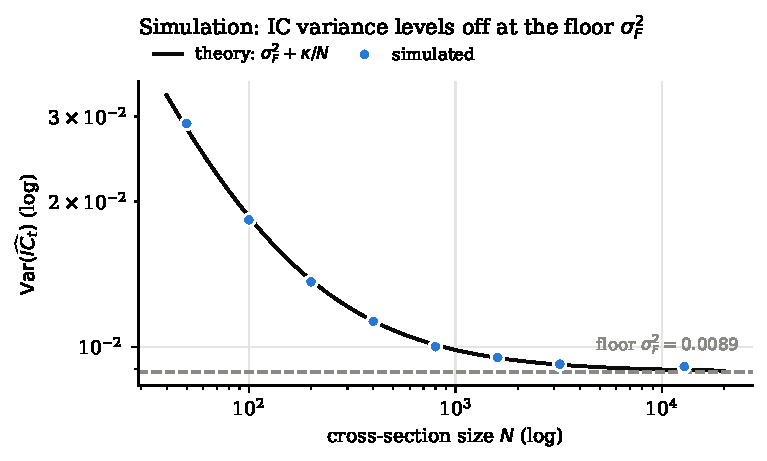
\includegraphics[width=0.78\textwidth]{figures/fig1_simulation.pdf}
\caption{Simulated IC variance against cross-section size, with the analytic curve
\eqref{eq:main} and the floor \eqref{eq:floor}. Variance falls as $1/N$ while the
idiosyncratic term dominates, then flattens.}
\label{fig:sim}
\end{figure}

The fitted coefficient on $1/N$ is $\simFitC \pm \simFitCSe$ where theory predicts
$\kappa = \simKappa$, a gap inside two Monte Carlo standard errors. The fit is unweighted
and so leans on the smallest $N$, where the $O(N^{-3/2})$ remainder still pushes $c$ up.


\paragraph{Which expression for the floor.}
The fitted intercept, $\simFit \pm \simFitSe$, is the simulated floor, and
Table~\ref{tab:floors} compares it with the exact form \eqref{eq:floor} and the two
closed forms \eqref{eq:closedforms}. The exact form is $\simExactErr\%$ away, within
Monte Carlo error. The closed form that keeps $v_\beta\sigma_f^2$ in the denominator is
$\simClosedErr\%$ too high, and dropping that term makes it worse.

\begin{table}[htbp]
\centering
\begin{tabular}{lrrr}
\toprule
estimator & value & error & Monte Carlo $\sigma$ \\
\midrule
exact leading order, \eqref{eq:floor}        & \simFloor  & $+\simExactErr\%$  & $\simExactSig$ \\
closed form $q^2\sigma_f^2/(\sigma_\varepsilon^2 + v_\beta\sigma_f^2)$ & \simClosed & $+\simClosedErr\%$ & $\simClosedSig$ \\
naive ratio $q^2\sigma_f^2/\sigma_\varepsilon^2$ & \simNaive  & $+\simNaiveErr\%$  & $\simNaiveSig$ \\
\bottomrule
\end{tabular}
\caption{Candidate expressions for $\sF^2$ against the simulated floor
$\simFit \pm \simFitSe$. Only the exact leading-order expression is within two Monte
Carlo standard errors of it.}
\label{tab:floors}
\end{table}

\paragraph{Coverage and power.}
For Table~\ref{tab:cov} I draw $2{,}000$ samples of $T$ periods each at $N = 400$. In
each sample I record whether the Fama--MacBeth interval covers the true mean IC and
whether the test rejects $\rho = 0$. From $T = 60$ on, coverage is within a percentage point of
$95\%$ and simulated power is within about $0.015$ of the analytic value, which supports
using \eqref{eq:reqT} for the sample-size calculations in \S\ref{sec:implications}. At
$T = 24$ both are off by about three Monte Carlo standard errors, for the reason given in
the caption.

\begin{table}[htbp]
\centering
\begin{tabular}{rrrr}
\toprule
$T$ & coverage of $95\%$ interval & power, simulated & power, analytic \\
\midrule
24  & \covtwofour       & \pwsimtwofour       & \pwanatwofour \\
60  & \covsixzero       & \pwsimsixzero       & \pwanasixzero \\
120 & \covonetwozero    & \pwsimonetwozero    & \pwanaonetwozero \\
300 & \covthreezerozero & \pwsimthreezerozero & \pwanathreezerozero \\
\bottomrule
\end{tabular}
\caption{Coverage and power at $N = 400$, true mean IC $\simTrueIC$. At $T = 24$ the
simulated power is a little above the analytic value, and coverage a little below
$95\%$, because the test uses a normal critical value where a $t$ distribution with few
degrees of freedom would be more accurate.}
\label{tab:cov}
\end{table}

\section{Data}\label{sec:data}

The stock list is the holdings of the iShares Russell 3000 ETF (IWV) on the day the data
were downloaded, with sectors taken from the same holdings file. Daily prices for those
stocks come from Yahoo Finance, downloaded with the open-source \texttt{yfinance} library.
The result is one file (\texttt{russell3000\_data.csv}) with daily open, high, low, close,
volume and sector for \nTickers{} US tickers, $11{,}262{,}530$ rows spanning 2000-01-03 to
2026-03-11. Closes are
back-adjusted for splits and dividends, so successive ratios are total returns. I take
the last observed close in each calendar month, form monthly returns, and discard the
final partial month, giving $313$ months from \panelStart{} to \panelEnd{}. The momentum sample has a
median of $\momN$ names per month.

Two signals are constructed, both from prices alone: $12-1$ momentum, the cumulative log
return over the eleven months ending one month before formation
\citep{jegadeesh1993returns}, and one-month reversal, the previous month's return
negated \citep{jegadeesh1990evidence}. Signals are measured at the end of month $t$ and
matched to the return earned during month $t+1$.

\paragraph{Known defects.}
The data has three known problems, and I checked each one directly
(Appendix~\ref{app:audit}). \emph{(i) The universe is completely survivorship-biased.}
All \nTickers{} tickers survive to the final date, with no
delistings. This follows from how the file was built: the stock list is the index's
membership on the download date, so any company that left the index earlier, through
bankruptcy, a merger or deletion, is not in the data. \emph{(ii) Some columns are
transformed despite their names.} In an
accompanying fundamentals file, a column named \texttt{book\_to\_market} is $83.2\%$
negative and its exponential has median $0.447$: it is log book-to-market. A column named
\texttt{div\_yield} takes only the values $\{0,1,2,3\}$. I use neither file; this check
is one reason the analysis uses prices only. \emph{(iii) The price snapshot cannot be
rebuilt exactly}, since every later dividend rescales the back-history. Testing this
would mean downloading the data again, which I did not do, so my original download is
the input of record. I also checked that every close lies inside that day's high-low
range, which suggests that closes and the other prices are adjusted the same way.

Section~\ref{sec:limitations} discusses what defect (i) means for the results.

\section{Empirical results}\label{sec:empirical}

\subsection{The realised IC series}

\begin{table}[htbp]
\centering
\begin{tabular}{lrrrrrrrr}
\toprule
signal & $T$ & mean & sd & $t$ & $t_{NW}$ & AR(1) & median $N$ & $\Neff$ \\
\midrule
$12-1$ momentum   & \momT & \momMean & \momSd & \momTstat & \momTnw & \momAR & \momN & \momNeff \\
1-month reversal  & \revT & \revMean & \revSd & \revTstat & \revTnw & \revAR & \revN & \revNeff \\
\bottomrule
\end{tabular}
\caption{Monthly Spearman IC, \panelStart{} to \panelEnd{}. $t$ is the Fama--MacBeth
statistic $\sqrt{T}\,\overline{IC}/\hat\sigma_{IC}$; $t_{NW}$ applies a Newey--West
correction with six lags.}
\label{tab:series}
\end{table}

Momentum's mean IC of $\momMean$ carries $t = \momTstat$: not distinguishable from zero.
Under the classical formula it would have been overwhelming, since $\iidNull/\sqrt{\momT}
= 0.0015$ implies $t \approx 8$. Reversal's $\revMean$ gives $t = \revTstat$, which
survives even the $t > 3$ hurdle of \citet{harvey2016cross}. Autocorrelation is
negligible in both ($\momAR$ and $\revAR$), so the Newey--West correction moves the
statistics only slightly, and upward: $\momTnw$ and $\revTnw$.

\subsection{IC volatility and breadth}

Proposition~\ref{prop:main} makes a prediction that can be tested on real data without
specifying any factor model. Draw random subsets of $N$ names, recompute the IC series,
and see whether its variance traces $\sF^2 + c/N$ with $c = 1$. Only $26\%$ of months
have $2{,}000$ names, all of them late in the sample, so the subsamples stop at
$N = 1000$. The thinnest month has $1{,}083$ names, so every month enters at every size.

\begin{table}[htbp]
\centering
\begin{tabular}{rrrrr}
\toprule
$N$ & $12-1$ momentum & 1-month reversal & random signal & classical $1/\sqrt{N-1}$ \\
\midrule
\breadthrows
\bottomrule
\end{tabular}
\caption{Standard deviation of the realised IC series by cross-section size, averaged
over five independent draws. The random signal is a per-period random permutation:
it has $q = 0$ by construction. Its fitted floor is $\randFloorVar$, essentially zero,
against momentum's $\momFloorVar$.}
\label{tab:breadth}
\end{table}

\begin{figure}[htbp]
\centering
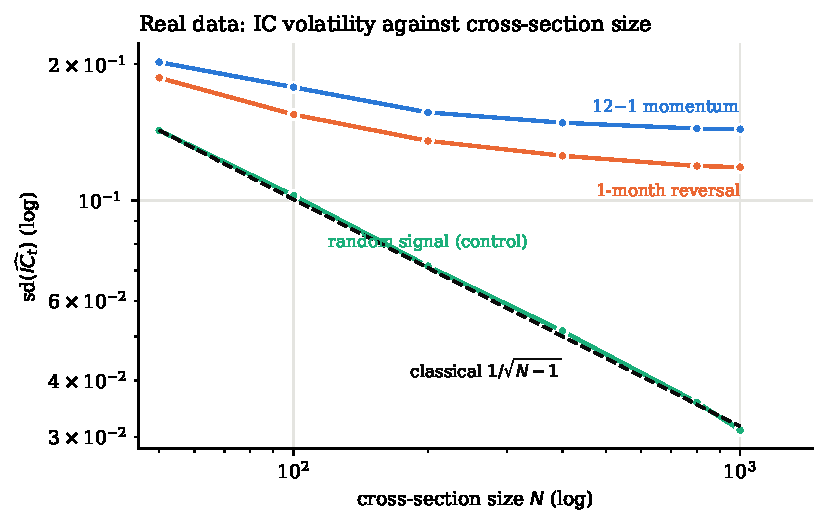
\includegraphics[width=0.85\textwidth]{figures/fig2_breadth.pdf}
\caption{IC volatility against cross-section size on real data. The random-signal control
lies on the classical curve throughout; both real signals flatten well above it.}
\label{fig:breadth}
\end{figure}

The fitted coefficient on $1/N$ is $\momC$ for momentum and $\revC$ for reversal,
against a predicted $1$, so the functional form fits. The overshoot of about
$\momOvershoot\%$ is larger than the random-signal control's ($\randC$ on the same
months). A likely reason is assumption (A3): residual returns are correlated within
industries, so the diversifiable term shrinks a little more slowly than $1/N$. That changes the
constant on $1/N$, not the floor.

The random-signal control follows $1/\sqrt{N-1}$ to within $\randMaxDev\%$ over a
twenty-fold range of $N$, with a fitted floor of $\randFloorVar$. If dependence between returns were enough to create the floor, a
structureless signal would show one too, and it does not. The floor needs $q \neq 0$, a
signal correlated with loadings, as \eqref{eq:decomposition} says. Because the
control goes through the same code as the real signals, it also checks the IC
estimator.

Momentum's IC volatility levels off at $\sF = \momFloor$, so by \eqref{eq:neff} the
ceiling on effective breadth is $\momCeil$ observations. The cross-section actually used
has $\momN$ names and delivers $\momNeff$.

\subsection{A null with realistic dependence}

A second estimate of the floor keeps both cross-sections intact and breaks only the
timing: each month's signal is paired with a \emph{different} month's returns. This
gives the distribution of the IC when there is no predictive relation at all but the
real factor structure is still there. A random permutation also creates a few pairs
that are not nulls: a month matched with itself, or with a return already inside the
signal's twelve-month look-back (for reversal these score exactly $-1$). Those pairs are
dropped. Momentum's placebo has standard deviation $\momPlacebo$, against $\iidNull$
from the classical formula, so it is about $\momPlaceboRatio$ times wider even though
predictability is exactly zero.

\begin{figure}[htbp]
\centering
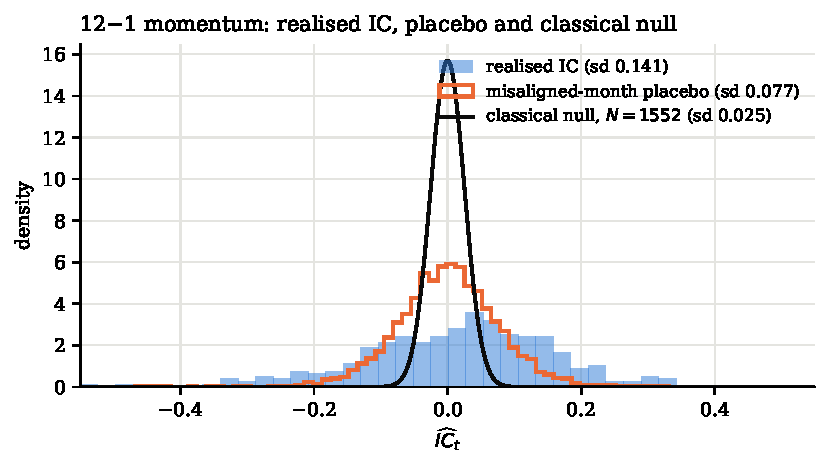
\includegraphics[width=0.85\textwidth]{figures/fig3_nulls.pdf}
\caption{Three distributions of the same statistic: the classical null, the
misaligned-month placebo, and the realised IC.}
\label{fig:nulls}
\end{figure}

This placebo is a \emph{lower} bound on $\sF$. Misaligning months also severs any link
between a signal's factor exposure in one month and factor volatility in the next, and if
those covary the placebo understates the floor. That is why I use the subsampling curve
as the main estimate and the placebo only as a check.

\begin{figure}[htbp]
\centering
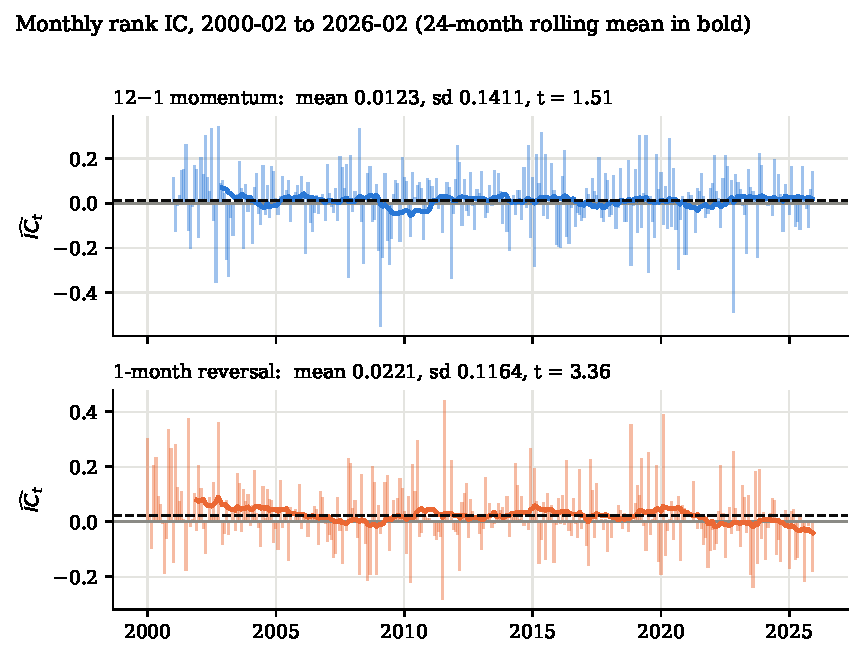
\includegraphics[width=0.88\textwidth]{figures/fig4_series.pdf}
\caption{The two realised monthly IC series with 24-month rolling means. The paper uses
their dispersion, not their level.}
\label{fig:series}
\end{figure}

\subsection{Robustness}

\paragraph{Rank versus raw correlation.}
My derivation is for Pearson correlation; I report Spearman. Computed both ways on
raw returns, momentum's IC standard deviation is $\momSd$ (Spearman) against
$\pearsonSd$ (Pearson), effectively identical, so the main result does not depend on
the rank transform. The \emph{mean}, however, moves from $\momMean$ to $\pearsonMean$
and changes sign. The panel contains a monthly return of $+30{,}991\%$, and a point
estimate that a single observation can flip is not one to build on, which is why I
use ranks.

\paragraph{Survivorship.}
Restricting the sample to the $\cohortN$ tickers with closes at the end of both January
and February 2000 (the first monthly return), a cohort
with a different survivorship pattern, moves the mean IC from $\momMean$ to
$\cohortMean$ (about a third of its value), while the standard deviation moves from
$\momSd$ to $\cohortSd$, about $\cohortSdChange\%$. The paper relies on the second moment
being stable, and here it is much more stable than the first.

\section{Implications}\label{sec:implications}

\paragraph{How much data a claimed IC of $0.03$ needs.}
At the measured $\sigma_{IC} = \sigmaIC$, equation \eqref{eq:reqT} at $80\%$ power gives:

\begin{table}[htbp]
\centering
\begin{tabular}{lrr}
\toprule
hurdle & required $T$ (months) & years \\
\midrule
$t > 1.96$, single test                       & \reqTsingle & \reqYsingle \\
$t > 3.00$ \citep{harvey2016cross}            & \reqThlz    & \reqYhlz \\
$t > 3.76$, Bonferroni over $300$ anomalies   & \reqTbonferronithreezerozero & \reqYbonferronithreezerozero \\
\bottomrule
\end{tabular}
\caption{Sample length required to distinguish a true IC of $0.03$ from zero.}
\label{tab:reqT}
\end{table}

A study using the CRSP sample from 1963 to about 2020 ($\approx 57$ years) clears the single-test bar
comfortably and the multiple-testing bar with room. A study on twenty years of one
country's data, or on a subperiod, or on any market with a short history, does not.

\paragraph{Decade-by-decade claims.}
Equation \eqref{eq:mde} gives the smallest IC detectable at $80\%$ power:

\begin{center}
\begin{tabular}{lrrrrr}
\toprule
sample length & 5 yr & 10 yr & 20 yr & 25 yr & 57 yr \\
\midrule
$\rho_{\min}$ & \mdefive & \mdeonezero & \mdetwozero & \mdetwofive & \mdefiveseven \\
\bottomrule
\end{tabular}
\end{center}

\noindent
Over ten years the minimum detectable IC is $\mdeonezero$, larger than $0.03$, so a paper that reports a mean IC of $0.03$ \emph{and} claims the effect holds in every
decade is claiming something its decade-long windows cannot establish at conventional
power. Either the subperiod results are underpowered and their significance is partly
luck, or the true IC is larger than $0.03$. Subperiod robustness tables are common, and
this objection can be checked against any of them.

\begin{figure}[htbp]
\centering
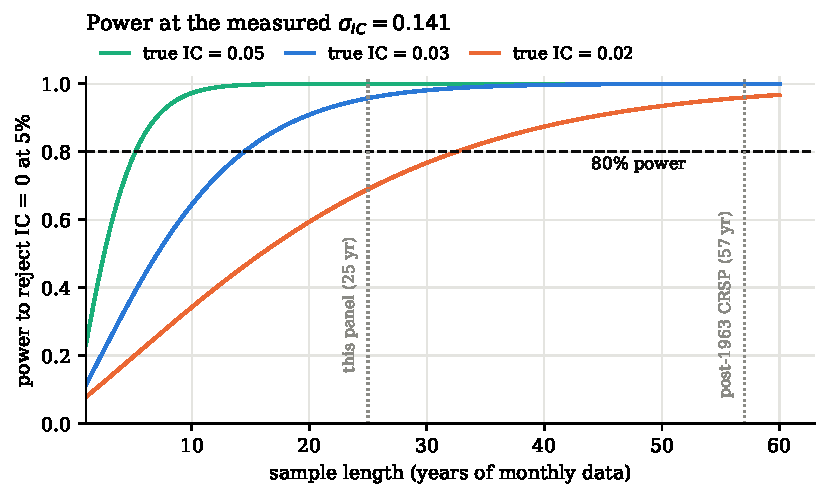
\includegraphics[width=0.85\textwidth]{figures/fig5_power.pdf}
\caption{Power to reject $IC = 0$ against sample length, at the measured
$\sigma_{IC} = \sigmaIC$.}
\label{fig:power}
\end{figure}

\paragraph{Effective size of the panel.}
The panel contains \panelObs{} stock-months. By \eqref{eq:effobs} it carries \effObs{}
effective observations, about \overstate{} times fewer, against the \neededObs{} needed
to detect an IC of $0.03$ at $80\%$ power. Twenty-five years of a broad universe clears
that bar by less than a factor of two.

\paragraph{Exaggeration.}
Evaluating \eqref{eq:typem} at $\sigma_{IC} = \sigmaIC$ for a true IC of $0.03$:

\begin{center}
\begin{tabular}{lrrrrr}
\toprule
sample length & 5 yr & 10 yr & 20 yr & 25 yr & 57 yr \\
\midrule
exaggeration ratio & \typemfive & \typemonezero & \typemtwozero & \typemtwofive & \typemfiveseven \\
\bottomrule
\end{tabular}
\end{center}

\noindent
The winner's curse here is a short-sample problem. At five years a published IC of this
size is inflated by about $\typemfive\times$, and by twenty-five years the effect is
negligible. The result therefore
supports the claim that low power inflates estimates from short samples and subperiods,
but not long-sample anomaly estimates in general.

\begin{figure}[htbp]
\centering
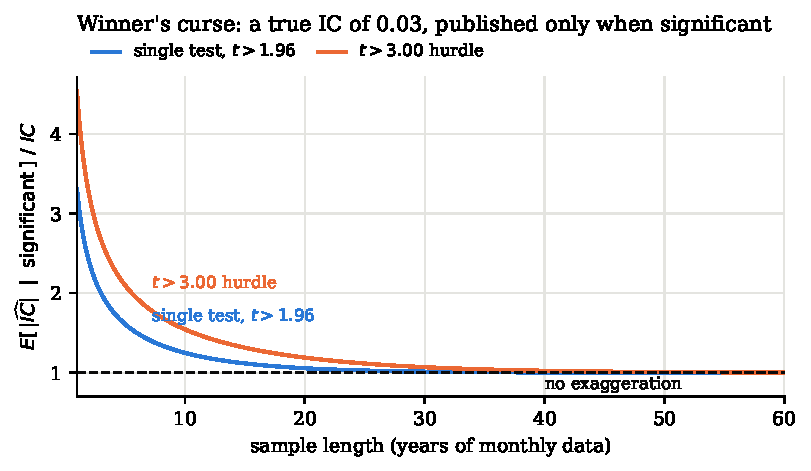
\includegraphics[width=0.85\textwidth]{figures/fig6_typem.pdf}
\caption{Exaggeration ratio for a true IC of $0.03$ reported only when significant.}
\label{fig:typem}
\end{figure}

\paragraph{What the results do not show.}
None of this means published anomalies are false; \citet{chen2021phacking} argues that
the largest published $t$-statistics cannot be produced by $p$-hacking alone. What the results do show is that a cross-sectional IC is much less
precise than the size of the panel suggests, that the shortfall can be calculated in
advance, and that a small IC from a short sample
should be treated as underpowered until shown otherwise.

\section{Limitations}\label{sec:limitations}

\paragraph{The universe is completely survivorship-biased.}
This is the most serious limitation and it cannot be repaired with the data available.
All \nTickers{} tickers survive to the end, because the stock list is the index's
membership on the download date; a point-in-time universe would have several
times as many names and thousands of delistings, and the bias is not constant over time.
My mean ICs are therefore not credible estimates of any economic quantity, and I do not
present them as such. The paper's claims concern $\sigma_{IC}$ and $\Neff$, which are
second moments and much less exposed. The cohort test in \S\ref{sec:empirical} supports this
without proving it. A fully point-in-time
panel could give a different $\sF$, most plausibly a larger one, since delisting returns
are volatile and cross-sectionally clustered in exactly the periods when factor
realisations are extreme.

\paragraph{One market, one sample period, two signals.}
Everything is US equities, \panelStart{}--\panelEnd{}, price-based signals. I have not
shown that $\sF \approx \momFloor$ generalises to other markets, longer histories, or
accounting-based signals. The \emph{mechanism} should generalise wherever a signal
correlates with factor loadings, but the magnitude is an empirical quantity and I
measured it once.

\paragraph{The simulation's IC is thin-tailed; real ICs are not.}
As noted after Proposition~\ref{prop:main}, $g(f)$ is bounded, so the simulated IC has
lighter tails than a normal. The realised series have kurtosis about $\momKurt$, slightly
heavy. The coverage figures in Table~\ref{tab:cov} are therefore mildly optimistic
relative to real data, and inference on real IC series is likely to be slightly worse
than the simulation suggests.

\paragraph{The model is simple.}
One factor, constant loadings, cross-sectionally uncorrelated residuals. Residual
correlation from industry clustering would add a further non-diversifiable term, so
relaxing (A3) worsens the conclusion. Time variation in $q$ or $\lambda$ likewise adds
variance. I am not aware of a plausible relaxation that makes precision better.

\paragraph{The snapshot is not exactly reproducible.}
Adjusted closes drift as dividends accumulate, so a fresh download from Yahoo Finance should not be
expected to match this file exactly. Returns computed from adjusted closes are still correct returns, so this limits exact
reproducibility but does not bias the results, which are stated against my original
download.

\section{Conclusion}

Past a modest number of stocks, the precision of a cross-sectional information
coefficient depends on the number of periods and hardly at all on the number of stocks.
Any usable signal is correlated with factor loadings, so each period's IC absorbs the
realised factor return, one draw common to every name, and adding stocks does not
average it away. The per-period variance is $\sF^2 + \kappa/N$ with $\kappa \approx 1$,
effective breadth is capped at $1/\sF^2$, and the required sample length follows
directly.

Measured on \nTickers{} US stocks over twenty-five years, $\sF = \momFloor$, so a
cross-section of $\momN$ names is worth about $\momNeff$ independent observations and
the whole panel is worth \effObs{} observations, not \panelObs{}. Detecting a true IC of
$0.03$ needs \reqYsingle{} years for a single test and \reqYhlz{} years at the hurdle the
field has adopted, and no ten-year window can detect it at all. My own momentum series
gives $\momMean$ with $t = \momTstat$, which I report as a null.

The per-period floor is not new; it is strategy risk \citep{qian2004active} and it bounds
the attainable information ratio \citep{ding2017redux}. What this paper adds is reading
it as a statement about statistical power: effective sample size, required $T$, and the
exaggeration of published magnitudes. The calculation is cheap and can be done before a
study is run.

\paragraph{Reproducibility.}
Code for every result in this paper is at
\url{https://github.com/thotahimalnaidu/ic-power-analysis}. The price data come from Yahoo
Finance and are not redistributed; \texttt{make download} fetches a fresh copy with
\texttt{yfinance}, which will differ slightly from mine for the reason given in
\S\ref{sec:limitations}.

\paragraph{Use of AI tools.}
I used an AI assistant (Claude, Anthropic) for initial planning, help with debugging,
language and grammar editing, presentation, and a final check of the manuscript. The
research question, derivation, data analysis and conclusions are my own. I take full responsibility for the content and any errors.

\bibliographystyle{plainnat}
\bibliography{refs}

\appendix

\section{Proof of Proposition \ref{prop:main}}\label{app:proof}

\paragraph{Conditional on the factor draw, the cross-section is i.i.d.}
Fix $f \equiv f_{t+1}$. By (A6), each asset's $(s_i, \beta_i, \varepsilon_i)$ is an
independent draw from the same joint normal distribution, and
$r_i = \lambda s_i + \beta_i f + \varepsilon_i$ is linear in that draw. So conditional
on $f$ the pairs $(s_i, r_i)_{i=1}^{N}$ are an i.i.d. sample from a bivariate normal
distribution with correlation
\begin{equation*}
\mathrm{corr}(s, r \mid f) \;=\; \frac{\lambda + qf}{\sqrt{\sigma_\varepsilon^2 + v_\beta f^2 + \lambda^2 + 2\lambda qf}} \;=\; g(f).
\end{equation*}
All of the dependence across assets runs through $f$, so once $f$ is fixed the
\emph{classical} formula \eqref{eq:classical} applies as it stands:
\begin{equation}
\mathrm{Var}(\ICh_t \mid f) \;=\; \frac{\left(1 - g^2\right)^2}{N} + O(N^{-3/2}),
\qquad
\mathrm{E}[\ICh_t \mid f] \;=\; g - \frac{g\left(1 - g^2\right)}{2N} + O(N^{-3/2}),
\label{eq:conditional}
\end{equation}

\paragraph{Law of total variance.}
\begin{align*}
\mathrm{Var}(\ICh_t)
&= \mathrm{Var}_f\!\left[\mathrm{E}(\ICh_t \mid f)\right]
 + \mathrm{E}_f\!\left[\mathrm{Var}(\ICh_t \mid f)\right] \\[0.2em]
&= \underbrace{\mathrm{Var}_f\!\left[g\right]}_{=\;\sF^2}
 \;-\; \frac{1}{N}\,\mathrm{Cov}_f\!\left(g,\, g\left(1-g^2\right)\right)
 \;+\; \frac{1}{N}\,\mathrm{E}_f\!\left[\left(1-g^2\right)^2\right]
 \;+\; O(N^{-3/2}).
\end{align*}
The first term is \eqref{eq:floor} and does not involve $N$; the other two vanish as
$N \to \infty$ and together are $\kappa/N$ as defined in \eqref{eq:kappa}. The covariance
term comes from the conditional mean, which carries an $O(N^{-1})$ bias, and
because that bias moves with $f$ it contributes to the variance at order $1/N$. Writing
$\rho = \mathrm{E}_f[g]$ and using $\mathrm{E}_f[g^2] = \rho^2 + \sF^2$, both terms expand
to give $\kappa = 1 - 2\rho^2 - 3\sF^2 + O(g^4)$, which is $\simKappa$ in the calibration
of \S\ref{sec:simulation}. This gives \eqref{eq:main}. \hfill$\square$

\paragraph{Remark.} A derivation that tracks only the idiosyncratic term $u_t$
in \eqref{eq:numerator} gets $\sigma_\varepsilon^2/(N D(f)^2)$ for the
conditional variance, where $D(f)$ is the denominator of $g$ in \eqref{eq:floor}. It
misses the sampling error in $\mathrm{cov}_i(s,\beta)$ and in $\mathrm{sd}_i(r)$, which
are of the same order. In the calibration of \S\ref{sec:simulation} that route
understates the coefficient on $1/N$ by about $\simKappaUErr\%$. The simulation estimates this coefficient
from the data, which is how the error showed up. The $O(N^{-3/2})$ residual shows up in Table~\ref{tab:sim} as the slightly larger
errors at small $N$.

\section{The multi-factor statement}\label{app:multi}

With $K$ factors, $r_{i,t+1} = \lambda s_{i,t} + \boldsymbol\beta_i'\mathbf{f}_{t+1} +
\varepsilon_{i,t+1}$ and $\mathbf{q} = \mathrm{cov}_i(s, \boldsymbol\beta) \in
\mathbb{R}^K$, equation \eqref{eq:numerator} becomes
$\mathrm{cov}_i(s,r) = \lambda + \mathbf{q}'\mathbf{f}_{t+1} + u_t$ and the floor is
\begin{equation*}
\sF^2 = \mathrm{Var}_{\mathbf f}\!\left[
\frac{\lambda + \mathbf{q}'\mathbf{f}}
{\sqrt{\sigma_\varepsilon^2 + \mathbf{f}'V_\beta \mathbf{f} + \lambda^2
 + 2\lambda\mathbf{q}'\mathbf{f}}}\right],
\qquad V_\beta = \mathrm{cov}_i(\boldsymbol\beta, \boldsymbol\beta').
\end{equation*}
To leading order in small $\mathbf f$ this is $\mathbf{q}'\Sigma_{\mathbf f}\mathbf{q}/
\sigma_\varepsilon^2$. The floor is positive whenever the
signal loads on any priced or unpriced common factor, and it does not depend on $N$.

\section{Data checks}\label{app:audit}

The script \texttt{src/audit.py} checks the raw files directly. All $2{,}559$ tickers in
the price file have data on its final date, 2026-03-11, so there are no delistings. In
the fundamentals file, \texttt{book\_to\_market} is $83.2\%$ negative with median
$-0.805$, and its exponential has median $0.447$, which is what log book-to-market looks
like. \texttt{div\_yield} takes only the values $0$ to $3$, and $69\%$ of them are zero.
Every close in the price file lies within that day's high-low range, allowing for
floating-point rounding.

\end{document}
